% !TeX root = RJwrapper.tex
\title{\emph{countfitteR}: a web server for the analysis of count data}
\author{by Jaros\l{}aw Chilmoniuk, Madeleine Ruhe, Stefan R\"{o}diger and Micha\l{} Burdukiewicz}

\maketitle

\abstract{
countfitteR is a package designed for the analysis of count data and for determination of the best possible distribution, since overdispersion has severe impact on data analysis. It comes with easy to use shiny gui and webserver, providing clinical scientists simple interface for the analysis of the data, without biostatistical knowledge about nature of distributions. \\
In countfitteR we implemented 4 models of distribution. Poisson, which is typically used for count data, Negative Binomial (NB) dealing with extreme values, Zero-Inflated Poisson to depict Poisson-distributed data with excessive zeros and Zero-Inflated Negative Binomial to take care of increased variability of counts and zero-inflation. It can fit counts to mentioned distributions separately or globally, depending on the source of the data.
}

\section{ToDo}

\begin{itemize}
 \item Hurdle Model (Hu,M.-C. et al. (2011) Zero-Inflated and Hurdle Models of Count Data with Extra Zeros: Examples from an HIV-Risk Reduction Intervention Trial. The American Journal of Drug and Alcohol Abuse, 37, 367–375.)
\end{itemize}


\section{1. Introduction.}
\section{What is count data? | prevelence of count data}
Count data is a type of data in which the number of occurrences in a fixed period of time can take only the non-negative integer values.
This type of data is often found to .... and DNA double-strand breaks (DSB).

We developed a system that facilitates the digital  enumeration of DSBs via the phosphorylated histone  variant H2AX ($\gamma H2AX$), which is an important  biodositometer during radiation treatment. $\gamma H2AX$ is an important biomarker of physiological and pathological cellular processes \cite{reddig_dna_2018,rodiger_quantification_2018}. In addition, associated biomarkers such as the p53-binding protein 1 (53BP1) may also be detected during the screening. The foci quantification is a fast and sensitive approach for detection of one of the critical types of DNA damage introduced by radiation, cellular process or toxic agent with applications in research and clinical environment (e.g., individual radiosensitivity). Although these biomarkers play a crucial role in diagnostics, their levels vary not only between patients but also between replicates.

The Poisson model is typically used for count data. However, in the context of DSBs, real foci data often do not satisfy constraints implied by this distribution. This suggests that another probability distribution for positive integers may describe a data set more accurately. Therefore, an identification of the probability distribution of $\gamma H2AX$ foci and associated biomarkers is vital for the precise estimation of the mean number of foci per cell and its confidence intervals.


\section{why not always poisson? overdispersion}

Overdispersion is an important concept in the analysis of the data. It occurs when the variation is much higher than we would expect. Usually when this happens we try to fit our dataset to distribution model in order to get the sample mean as close as possible to population mean. Some distribution models have an attribute to fit variabilities of observations.

% Overdispersion may be caused by the increased variability of counts, for example when a counting algorithm under- and overcounts. In such situation the data might have the NB distribution. The other cause of overdispersion is called zero-inflation and occurs in datasets, where some factor introduced faulty zeros. That means that some counts, regardless of their real state, are treated as zeros. In this case, data has the ZIP distribution. If both faulty zeros and increased variance affect the data, the ZINB distribution is the most appropriate.\\
% Count data is commonly assumed to be Poisson-distributed. One of the important features of the Poisson distribution is the equality of variance and expected value. But often we encounter overdispersed datasets, when the variance is bigger than the mean, and the commonly used model does not have attribute to fit variabilities of observations as close as possible to population mean.\\
% That is why we implemented four distributions in countfitteR: Poisson (POIS), Zero-Inflated Poisson (ZIP), Negative Binomial (NB) and Zero-negative Binomial (ZINB) model overdispersed counts.

Most statistical tests developed for determining if data is Poisson-distributed, test the equality of variance and mean. The data is considered overdispersed when the variance is significantly higher than the mean. We consider two possible causes for overdispersion. Firstly, the extreme values (both very high and very low counts) may occur more often than it is assumed in the Poisson distribution. Such situations are well modeled by the negative binomial (NB) distribution. Despite the fact that the NB distribution is used primarily for counting the number of failures before a predetermined number of successes occurs, it can be also alternatively parametrized to describe count data with non-equal variance and mean. One of the important properties of the NB distribution is that the maximum likelihood (ML) estimator of its mean ($\hat{\mu}$) (e.g., the mean number of foci per cell) is equal to the arithmetic mean of counts in a data set.

The second cause of overdispersion is zero-inflation, an excessive number of zeros in a data set. We distinguish two causes for zero-inflation: either zeros occur naturally or false zeros are introduced by an unknown factor (e.g., foci not detected by the system). To describe zero-inflation we use the Zero-Inflated Poisson (ZIP) and the Zero-Inflated Negative Binomial (ZINB) distributions. The former is used to depict Poisson-distributed data, where overdispersion is caused by the excessive zeros and the latter for data where overdispersion arises from both increased variability of counts and zero-inflation. It is important to note, that in case of zero-inflated distributions, the mean number of counts $\lambda$ is not equal to the average number of foci per cell ($\mu$). To describe their relationship, we need to introduce another parameter, r, which is equal to the fraction of counts faulty turned to zeros. Using the introduced notation: $\lambda = \frac{\mu}{1 - r}$. Henceforth, if we do not correctly identify zero-inflation, we underestimate the real number of foci per cell.

Overdispersed distributions in most cases have variance larger than the Poisson-distributed counts with the same average number of foci per cell ($\lambda$). In consequence, the confidence intervals are wider than in the case of the Poisson distribution. It directly affects the conclusion drawn from a data analysis, because bigger change of the mean number of foci is required, to support the significance of the impact of the treatment. 

Since overdispersion has serve impact on a data analysis, we created \emph{countfitteR} for determination of the count data distribution. Our software fits count data to four distributions, that describe counts: Poisson, NB, ZIP and ZINB. Although statistical tests designed for detecting overdispersion exist, they work properly only in a specific range of values. Furthermore, these tests only indicate that data is overdispersed, but do not point the suitable probability distribution. Therefore, \emph{countfitteR} selects the appropriate model using the Bayesian Information Criterion (BIC). The analysis is coupled with an estimation of parameters in the distribution of choice and their confidence intervals.  


%####################################### New section?, need to format

Parameters:

* $\lambda$ - Poisson parameter (average number of foci per cell).  
* $r$ - zero inflation (fraction of cells treated by system as having no foci regardless of their real state).  
* $\theta$ - dispersion parameter.
  
Usually the NB distribution is parameterized using $\mu$ and $\theta$, but to make comparison clearer, we use $\lambda$ instead of $\mu$. In this parameterization, NB and ZINB are treated as the mixture of Poisson and Gamma ($\Gamma$) distributions.  

Distribution <br> name  | pmf 
-------------------|-------------
Poisson            |$$P\{X = k\} = \frac{\lambda^k \exp^{-\lambda}}{k!} $$
Zero-inflated Poisson                |$$P\{X = k\} = \begin{cases} r + ( 1- r) \exp^{-\lambda},\text{if } k = 0\\ r \frac{\lambda^k \exp^{-\lambda}}{k!},\text{if } k = 1, 2, \ldots \end{cases} $$
Negative Binomial                 |$$P\{X = k\} = \frac{\Gamma (\theta + k)}{\Gamma(\theta) k!}  \left(\left( \frac{\theta}{\theta + \lambda} \right)^\theta \left( \frac{\lambda}{\theta + \lambda} \right) \right)^k$$
Zero-inflated Negative Binomial               |$$P\{X = k\} = \begin{cases}r + (1 - r) \left( \frac{\theta}{\theta + \lambda} \right)^\theta,\text{if } k = 0\\(1 - r) \frac{\Gamma (\theta + k)}{\Gamma(\theta) k!}  \left(\left( \frac{\theta}{\theta + \lambda} \right)^\theta \left( \frac{\lambda}{\theta + \lambda} \right) \right)^k,\text{if } k = 1, 2, \ldots\end{cases}$$

Poisson and Negative Binomial distributions have the same expected value. In case of ZIP and ZINB, the expected value is smaller than the real average number of foci per cell.

Distribution <br> name  | Expected value
-------------------|-------------
Poisson            |$$E(X) = \lambda $$
ZIP                |$$E(X) = (1 - r) \lambda $$
NB                 |$$E(X) = \lambda $$
ZINB               |$$E(X) = (1 - r)  \lambda $$ 

Depending on the value of $r$ the variance of ZIP and ZINB may be smaller or bigger than the variance of Poisson distribution. In case of the NB distribution, the variance is always bigger than for the Poisson distribution, although the difference becomes negligible, when the $\theta$ is much bigger than $\lambda^2$.

Distribution <br> name  | Variance
-------------------|-------------
Poisson            |$$\textrm{var}(X) = \lambda $$
ZIP                |$$\textrm{var}(X) = \lambda (1 - r)(1 + \lambda r)$$
NB                 |$$\textrm{var}(X) = \lambda + \frac{\lambda^2}{\theta} $$
ZINB               |$$\textrm{var}(X) = (1 - r) \lambda \left( 1 + r\lambda  + \frac{1}{\theta} \right)$$



\section{2. Package - what's inside.}



\section{Describe briefly main functions}

\emph{countfitteR} provides clinical scientists with a simple interface for the analysis of count data regardless of their biostatistical knowledge about the nature of the distribution. The framework covers two most common situations. In the first approach, each count is separately fitted to all above mentioned distributions. This is preferable for situations, where counts come from various sources. The second approach relies on fitting globally all counts to a distribution. Such a model is appropriate among others for technical replicates.
Our software is open source and accessible also from the command-line level, it is suitable for integration into other analysis pipelines dealing with count data. Therefore, we anticipate that our finding will have a broader use. 
The web server is accessible under: 
\url{update me}

\section{show the foci example here}

In the present study we used count data from an image based study of $\gamma H2AX$ foci. Analysis of such foci data is a common task both in life sciences and in diagnostics applications. Though \emph{countfitteR} was initially developed for modeling count data from the AKLIDES system, it may be used for foci data from other systems. 

\section{Show he shiny gui}

Our application is available as a web server that may be used in an analysis of any kind count data, not only $\gamma H2AX$ and 53BP1. It is accompanied by an in-depth manual depicting the implemented framework and a rationale behind it. The guide covers both theoretical fundamentals and usage of \emph{countfitteR}, from a data import to a report generation.

\section{3. Results and conclusion.}



\section{show other count-based packages}

ShrinkBayes: a versatile R-package for analysis of count-based sequencing data in complex study designs.\\
COUNT \\
The Focinator \\ %no distribution?
FoCo: a simple and robust quantification algorithm of nuclear foci \\ %no distribution
AER \\
pscl \\
countreg: Count Data Regression \\
CountsEPPM 

\section{some showcases}



\section{Functions from the command line}

\emph{countfitteR} has the following main functions that can
be used from the command line:

\begin{itemize}
    \item \textit{compare\_fit} to compare something,
    \item \textit{fit\_counts} to count something and
    \item \textit{plot\_fitcmp} to plot something.
\end{itemize}

fitCounts \\
Estimates are presented in the table below along with the BIC values of their models.
Function is used to estimate the best distribution models for given data
Fit count is used to fit counts to different distribution models.
function is used to create a list of parameters characterizing chosen model. Those attributes are: 
\begin{itemize}
    \item lambda - Poisson parameter (average number of foci per cell). the estimated value of mean
    \item confint - lambda confidence intervals
    \item BIC - Bayesian Criterion Information, important criterion for model selection
    \item model - information of applied model
\end{itemize}

summaryFitlist \\
summary fitlist creates data frame from a list created by fit counts function with additional attributes as:
\begin{itemize}
    \item theta - dispersion parameter.
    \item r - zero inflation (fraction of cells treated by system as having no foci regardless of their real state).
\end{itemize}
Estimated coefficients of models (lambda for all distributions, theta for NB and ZINB, r for ZIP and ZINB).

compareFit and plotFitcmp \\
compare fit function compares empirical distribution of counts with the distribution defined by the model fitted to counts. 
plot fitcmp creates plot from compare fit results. 
Points indicate the real number of counts, while bars the number of counts estimated by a distribution.


\section{Data sets}

The data were prepared as described in \citep{rodiger_quantification_2018}.

\section{Another section}

This section may contain a figure such as Figure~\ref{figure:rlogo}.

\begin{figure}[htbp]
  \centering
  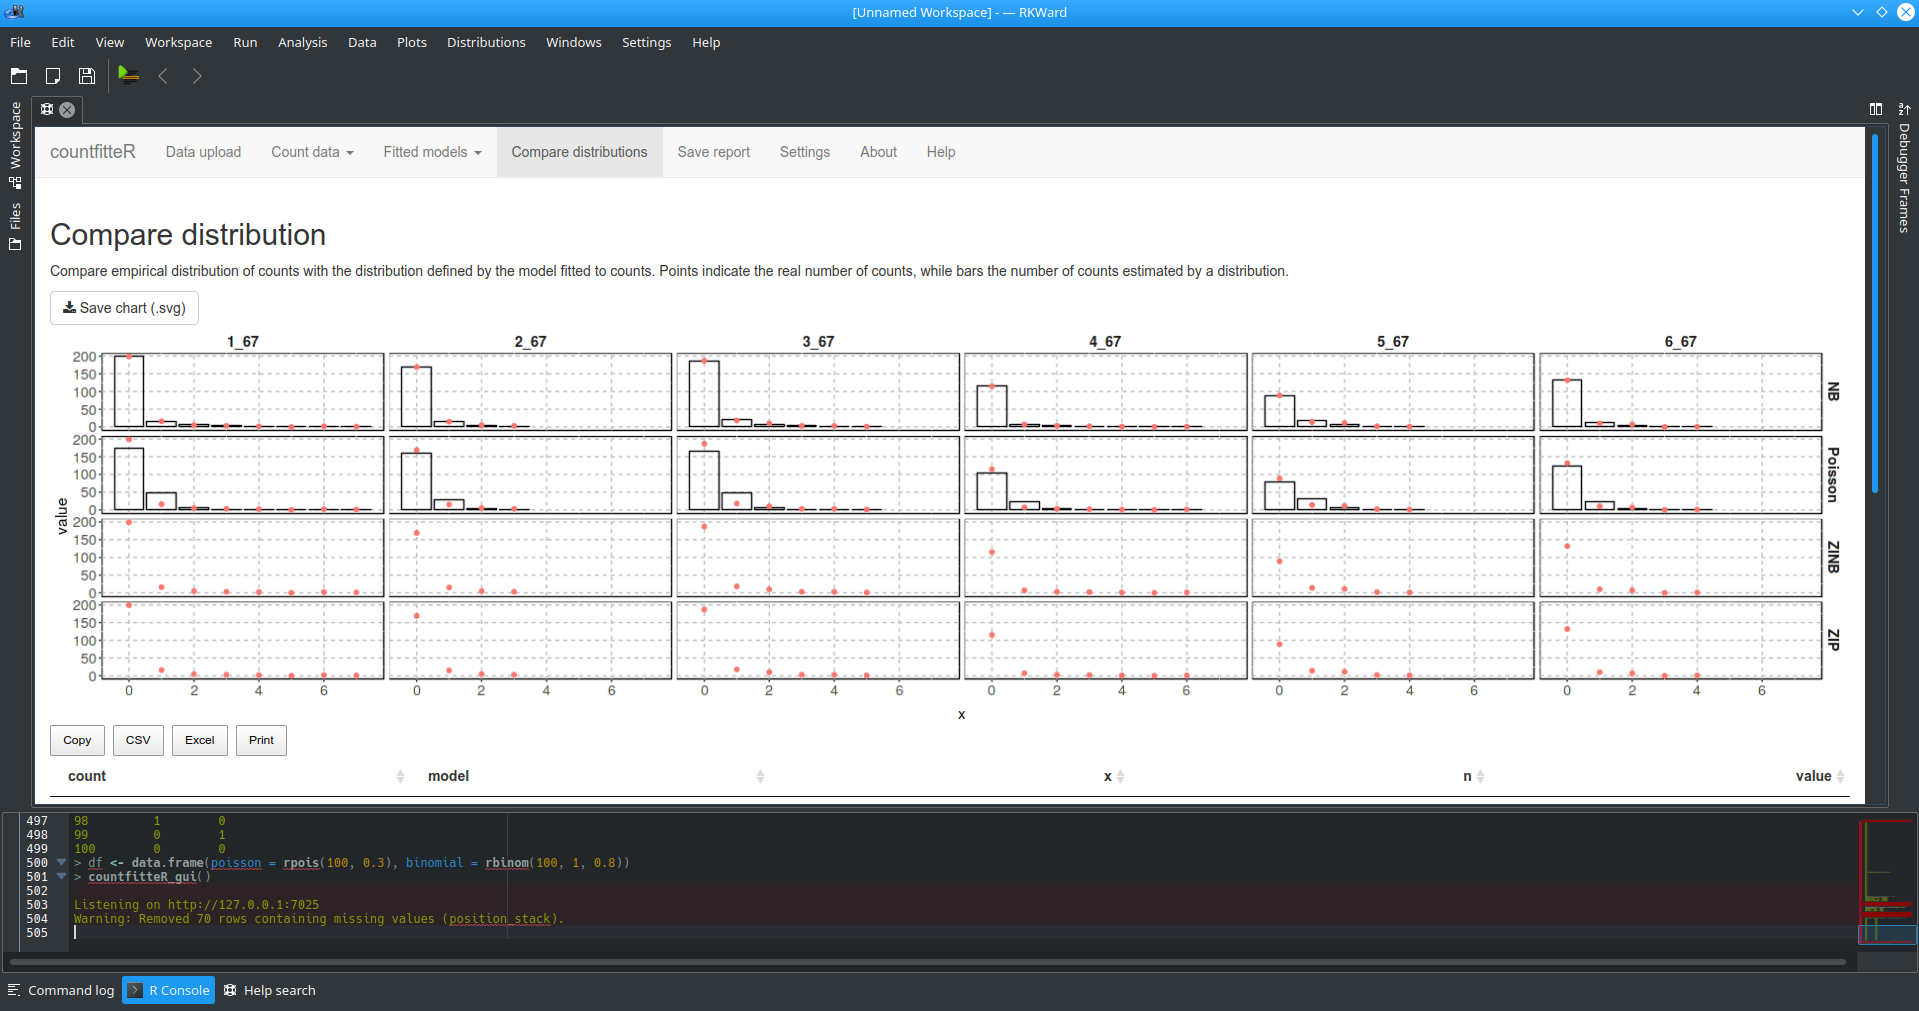
\includegraphics[width=0.99\columnwidth]{fig_gui}
  \caption{\emph{countfitteR} running in the \emph{RKWard} GUI/IDE \citep{rodiger_rkward:_2012}.}
  \label{figure:fig_gui.png}
\end{figure}

\section{Another section}

There will likely be several sections, perhaps including code snippets, such as:

\begin{example}
  x <- 1:10
  result <- myFunction(x)
\end{example}


\section{Summary}

This file is only a basic article template. For full details of \emph{The R Journal} style and information on how to prepare your article for submission, see the \href{https://journal.r-project.org/share/author-guide.pdf}{Instructions for Authors}.

\bibliography{Chilmoniuk}

\address{Jaros\l{}aw Chilmoniuk\\
  Affiliation\\
  Address\\
  Country\\
  (ORCiD if desired)\\
  \email{author1@work}}

\address{Madeleine Ruhe\\
  Brandenburg University of Technology Cottbus - Senftenberg\\
  Universit\"atsplatz 1, Senftenberg\\
  Germany\\
  (ORCiD if desired)\\
  \email{Madeleine.Ruhe1@b-tu.de}}

\address{Stefan R\"{o}diger\\
  Brandenburg University of Technology Cottbus - Senftenberg\\
  Universit\"atsplatz 1, Senftenberg\\
  Germany\\
  (ORCiD: 0000-0002-1441-6512)\\
  \email{stefan.roediger@b-tu.de}}

\address{Micha\l{} Burdukiewicz\\
  Affiliation\\
  Address\\
  Country\\
  (ORCiD: 0000-0001-8926-582X)\\
  \email{michalburdukiewicz@gmail.com}}
